\documentclass[journal]{IEEEtran}

\usepackage[T1]{fontenc}
\usepackage[utf8]{inputenc}
\usepackage{cite}
\usepackage{amsmath,amssymb}
\usepackage{booktabs}
\usepackage{siunitx}
\usepackage{hyperref}
\usepackage{enumitem}
\usepackage{balance}
\usepackage{tikz}
\usetikzlibrary{arrows.meta,positioning,shapes.geometric,fit}
\hypersetup{hidelinks}
\sisetup{detect-all=true}
\newcommand{\AirSense}{\textsc{AirSense-R}}

\begin{document}

\title{AirSense-R: Selection Reliability of PM$_{2.5}$ Forecasters Under Sensor Degradation and Site Shift}

\author{Daniel~Oyewale%
\thanks{Daniel Oyewale is affiliated with Ormedian Research Group. Corresponding email, funding, author-contribution, competing-interest, and data-availability statements will be finalized before submission.}}

\markboth{IEEE-Style Working Draft}{Oyewale: AirSense-R}
\maketitle

\begin{abstract}
Selecting an air-quality forecaster from clean validation accuracy does not establish whether that choice remains competitive when observations deteriorate or the monitoring site changes. We study this decision problem for one-hour-ahead PM$_{2.5}$ forecasting using hourly observations from 12 Beijing stations. Persistence, XGBoost, a multilayer perceptron (MLP), and a compact gated recurrent unit (GRU) network are compared under a frozen chronological protocol with training-only tuning, a predefined 1~$\mu$g/m$^3$ practical near-tie rule, and paired temporal-block uncertainty. Primary synthetic interventions cover non-target feature dropout, channel loss, measurement noise, and contiguous outages; historical PM$_{2.5}$ is not synthetically corrupted in this primary experiment. Site shift is evaluated through 12 leave-one-station-out folds. Although XGBoost has the lowest clean-test MAE (9.711~$\mu$g/m$^3$), the validation rule selects persistence, whose clean-test selection regret is 0.569~$\mu$g/m$^3$ (95\% CI: 0.340--0.763). Persistence remains within the practical threshold in all 15 full-period stress conditions under each imputation policy. Mean station-specific regret under site holdout is 0.550~$\mu$g/m$^3$ (95\% CI: 0.400--0.739), with 11 of 12 station point estimates within the practical threshold. A separately declared post-results extension probes the protected target-history assumption. Under a 12-hour PM$_{2.5}$ outage, affected-window regret rises to 2.282~$\mu$g/m$^3$ (95\% CI: 1.696--2.910), despite full-period regret of 0.651. These findings support a bounded conclusion: validation-based selection can remain practically competitive under many deployment stresses, but reliability depends on target-history availability and on whether evaluation is global or focused on affected windows.
\end{abstract}

\begin{IEEEkeywords}
PM$_{2.5}$ forecasting, model selection, selection regret, sensor degradation, missing observations, site shift, block bootstrap, reproducibility.
\end{IEEEkeywords}

\section{Introduction}
Ambient PM$_{2.5}$ remains a major environmental and public-health concern, with a substantial global disease burden attributable to long-term exposure~\cite{sang2022pm25burden}. Reliable short-horizon forecasting is therefore relevant to environmental monitoring and operational decision support. Yet a forecasting comparison ultimately produces a deployment decision, not merely a leaderboard.

That distinction matters because model rankings can change under missing data, measurement degradation, or distribution shift. A rank reversal alone, however, does not show that the original model choice has become materially poor. The deployment-relevant question is instead: \emph{how costly is it to retain the model selected under clean validation when operating conditions change?}

\AirSense{} studies that question through \emph{selection regret}: the excess forecasting error of the validation-selected family relative to the lowest-error candidate under the same evaluation condition. This paper does not introduce a new forecasting architecture. Its contribution is a reproducible empirical evaluation of a frozen accuracy-and-simplicity selection rule across clean testing, controlled input degradation, and unseen-station evaluation.

The study makes four contributions:
\begin{enumerate}[leftmargin=*,itemsep=2pt]
\item evaluation of a frozen validation-based selection rule across complementary deployment stresses;
\item interpretation of rank changes through selection regret, practical near-ties, and paired uncertainty;
\item a bounded post-results checkpoint that directly tests the protected PM$_{2.5}$ target-history assumption; and
\item an auditable evidence chain linking protocol, predictions, model lineage, uncertainty, and manuscript claims.
\end{enumerate}

The claims are deliberately bounded. We do not claim universal persistence superiority, a validated model-switching policy, robustness to physical sensor failure, or inter-city transfer.

\begin{figure*}[t]
\centering
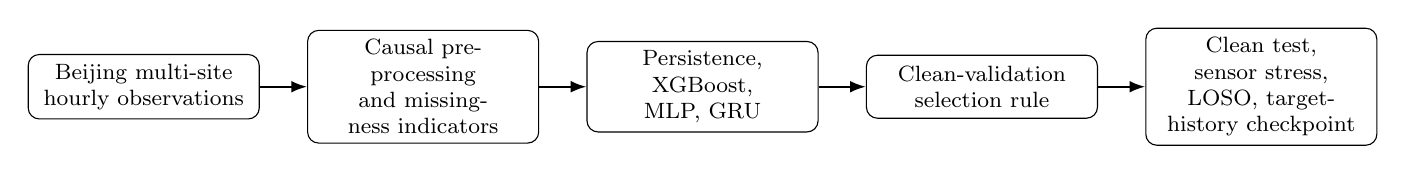
\begin{tikzpicture}[
node distance=5mm and 6mm,
box/.style={draw, rounded corners, align=center, minimum height=8mm, text width=2.7cm, font=\footnotesize},
arr/.style={-{Latex[length=2mm]}, thick}
]
\node[box] (data) {Beijing multi-site\\hourly observations};
\node[box, right=of data] (prep) {Causal preprocessing\\and missingness indicators};
\node[box, right=of prep] (models) {Persistence, XGBoost,\\MLP, GRU};
\node[box, right=of models] (select) {Clean-validation\\selection rule};
\node[box, right=of select] (stress) {Clean test, sensor stress,\\LOSO, target-history checkpoint};
\draw[arr] (data) -- (prep);
\draw[arr] (prep) -- (models);
\draw[arr] (models) -- (select);
\draw[arr] (select) -- (stress);
\end{tikzpicture}
\caption{AirSense-R study flow. The model-selection decision is frozen before downstream stress and site-shift evaluation.}
\label{fig:story}
\end{figure*}

\section{Related Work}
Air-quality forecasting under incomplete observations and spatial transfer is established research territory. Alvarado-Alcon \emph{et al.} study sparse sensor networks, cross-location generalization, and missing-data reliability~\cite{alvaradoalcon2026citywide}. Chowdhury \emph{et al.} show that imputation strategy can materially affect PM$_{2.5}$ prediction under incomplete sensor data~\cite{chowdhury2026imputation}. Liu \emph{et al.} examine PM$_{2.5}$ forecasting under temporal distribution shift and show that model behavior can depend on the evaluation regime~\cite{liu2024distshift}.

The closest methodological overlap is Semper \emph{et al.}~\cite{semper2026dss}, who study robust post-training model selection by reevaluating fixed prediction bundles against perturbed evaluation references. \AirSense{} instead perturbs the chronological \emph{input observation stream}, recomputes predictions, and separately evaluates station exclusion. This distinction supports cautious empirical positioning, not a claim to introduce selection regret or to be the first air-quality robustness study.

The candidate families intentionally span a simple persistence baseline, gradient-boosted trees~\cite{chen2016xgboost}, a feed-forward neural network, and a recurrent GRU model~\cite{cho2014gru}. The study is about selection reliability, not exhaustive architecture search.

\section{Data and Forecasting Task}
We use the UCI Beijing Multi-Site Air Quality dataset~\cite{uci_beijing}. The repository audit records 420,768 hourly rows across 12 monitoring stations, with 35,064 rows per station. The timestamp grid is complete, but measurements are not: accepted audit evidence records 8,739 missing PM$_{2.5}$ values (2.08\%) and 20,701 missing CO values (4.92\%).

The target is PM$_{2.5}$ concentration one hour ahead using the preceding 24 chronological hours. Numeric inputs are PM$_{2.5}$, PM$_{10}$, SO$_2$, NO$_2$, CO, O$_3$, temperature, pressure, dew point, rainfall, and wind speed; wind direction is categorical. Deterministic cyclical features encode hour-of-day and day-of-year. Station identity is used for grouping and exclusion, not as a predictor.

The chronological target splits are:
\begin{itemize}[leftmargin=*,itemsep=1pt]
\item training: 2 March 2013--28 February 2015;
\item validation: 1 March 2015--29 February 2016; and
\item final test: 1 March 2016--28 February 2017.
\end{itemize}
Missing targets are not imputed or scored, and synthetic interventions never alter the evaluation labels.

\section{Methods}
\subsection{Causal Preprocessing}
Each raw sensor channel receives a missingness indicator before imputation. Within each station, causal forward fill is limited to six consecutive hours. Remaining numeric gaps use medians estimated on fitting data only. Wind direction uses training-derived categories with explicit missing and unseen representations. MLP and GRU numeric inputs are standardized from training statistics after imputation; XGBoost receives unscaled numeric inputs.

A sensitivity policy removes forward fill while retaining training-only fallback and missingness indicators. The purpose is to test whether conclusions are primarily an artifact of causal carry-forward~\cite{chowdhury2026imputation}.

\subsection{Candidate Families}
Persistence predicts the next PM$_{2.5}$ value from the most recent causally preprocessed PM$_{2.5}$ observation. XGBoost operates on the 24-hour context as a tabular representation~\cite{chen2016xgboost}. The MLP provides a generic nonlinear neural baseline, while the compact GRU models the history sequentially~\cite{cho2014gru}. Learned families are tuned only within the training period; persistence has no tuning stage.

\subsection{Validation Selection}
Candidate families are evaluated on the same clean validation rows. The lowest aggregate validation MAE is identified. If another family lies within 1~$\mu$g/m$^3$ of the best, the difference is treated as a practical near-tie and the simpler family is preferred according to the fixed order
\[
\text{Persistence} \succ \text{XGBoost} \succ \text{MLP} \succ \text{GRU}.
\]
The selected family is frozen before final-test and stress outcomes are interpreted.

\begin{figure}[t]
\centering
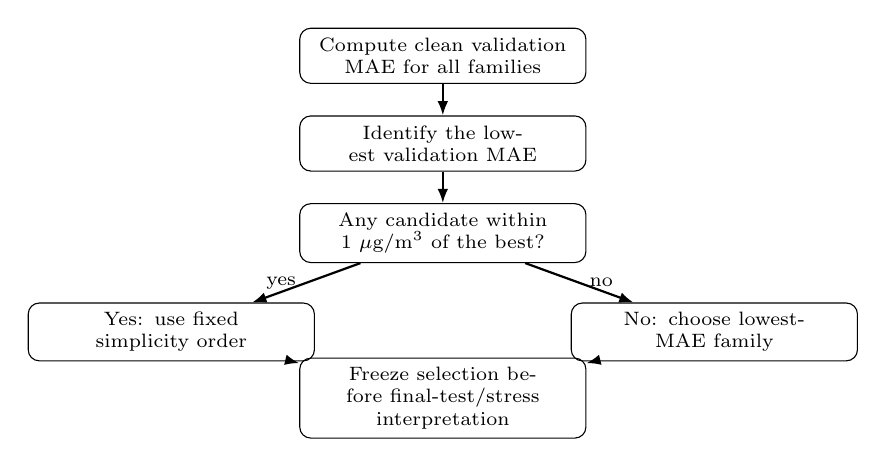
\begin{tikzpicture}[
node distance=4mm,
box/.style={draw, rounded corners, align=center, text width=3.4cm, minimum height=7mm, font=\scriptsize},
arr/.style={-{Latex[length=1.8mm]}, thick}
]
\node[box] (a) {Compute clean validation MAE for all families};
\node[box, below=of a] (b) {Identify the lowest validation MAE};
\node[box, below=of b] (c) {Any candidate within 1~$\mu$g/m$^3$ of the best?};
\node[box, below left=5mm and -2mm of c] (d) {Yes: use fixed simplicity order};
\node[box, below right=5mm and -2mm of c] (e) {No: choose lowest-MAE family};
\node[box, below=12mm of c] (f) {Freeze selection before final-test/stress interpretation};
\draw[arr] (a)--(b);
\draw[arr] (b)--(c);
\draw[arr] (c)--node[left,font=\scriptsize]{yes}(d);
\draw[arr] (c)--node[right,font=\scriptsize]{no}(e);
\draw[arr] (d)--(f);
\draw[arr] (e)--(f);
\end{tikzpicture}
\caption{Frozen validation-based selection rule.}
\label{fig:rule}
\end{figure}

For evaluation condition $s$, selection regret is
\begin{equation}
R_s = \mathrm{MAE}_s(m_{\mathrm{sel}})-\min_m\mathrm{MAE}_s(m),
\end{equation}
where $m_{\mathrm{sel}}$ is the validation-selected family. Regret measures model-choice cost relative to the available alternatives; it does not establish absolute operational adequacy.

\subsection{Primary Experiments}
The primary study has three components. First, all four candidates are evaluated on the untouched chronological final test. Second, frozen models are subjected to non-target input degradation: 10/30/50\% random feature dropout, whole-channel loss for NO$_2$, CO, and temperature, 5/10/20\% normalized measurement noise, and 6/12-hour outages for NO$_2$, CO, and temperature. Corruption is applied to the chronological stream before overlapping windows are constructed. Historical PM$_{2.5}$ is intentionally protected in this primary experiment.

Third, within-city site shift is evaluated through 12 leave-one-station-out folds. In each fold, the held-out station is excluded from preprocessing fitting, tuning, model fitting, and clean-validation selection. Recent local observations remain available at inference, so the task is unseen-station forecasting rather than uninstrumented spatial interpolation.

\subsection{Post-Results Target-History Checkpoint}
After the primary P5--P8 evidence had been inspected and preserved, a bounded extension was declared to probe the protected target-history assumption. The accepted models and preprocessing remain fixed. Exactly five conditions are tested: PM$_{2.5}$ dropout at 10, 30, and 50\%, and PM$_{2.5}$ contiguous outages of 6 and 12 hours. All candidates receive the same corrupted chronological stream before window construction; evaluation labels remain untouched. The extension is explicitly post-results and is reported separately from the original confirmatory evidence.

\subsection{Uncertainty and Reproducibility}
Paired uncertainty uses a 24-hour moving-block bootstrap with 2,000 replicates and shared temporal blocks across compared candidates, preserving short-range dependence better than treating hourly targets as independent~\cite{kuensch1989bootstrap}. The repository also preserves checksum-verified result manifests, executed notebooks, and read-only verification notebooks for accepted stages.

\begin{figure}[t]
\centering
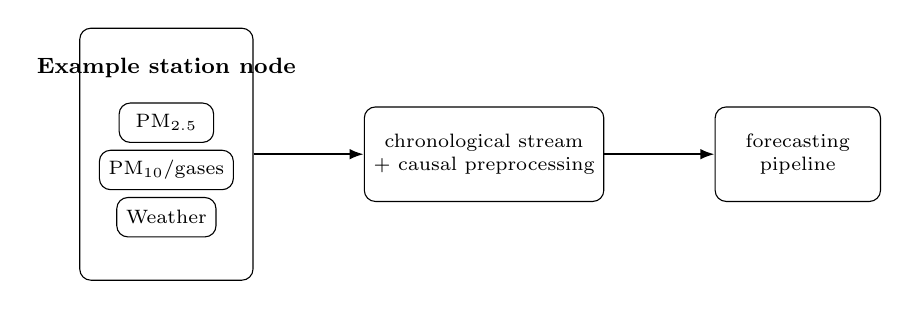
\begin{tikzpicture}[
font=\scriptsize,
sensor/.style={draw, rounded corners, minimum width=12mm, minimum height=5mm},
arr/.style={-{Latex[length=1.8mm]}, thick}
]
\node[draw, rounded corners, minimum width=2.2cm, minimum height=3.2cm] (node) {};
\node[font=\footnotesize\bfseries] at ([yshift=11mm]node.center) {Example station node};
\node[sensor] at ([yshift=4mm]node.center) {PM$_{2.5}$};
\node[sensor] at ([yshift=-2mm]node.center) {PM$_{10}$/gases};
\node[sensor] at ([yshift=-8mm]node.center) {Weather};
\node[draw, rounded corners, right=14mm of node, minimum width=2.2cm, minimum height=1.2cm, align=center] (pipe) {chronological stream\\+ causal preprocessing};
\node[draw, rounded corners, right=14mm of pipe, minimum width=2.1cm, minimum height=1.2cm, align=center] (forecast) {forecasting\\pipeline};
\draw[arr] (node)--(pipe);
\draw[arr] (pipe)--(forecast);
\end{tikzpicture}
\caption{Conceptual deployment context. The study evaluates forecasting behavior under degraded observation streams; it does not validate a specific physical sensor device.}
\label{fig:device}
\end{figure}

\section{Results}
\subsection{Clean Benchmark}
XGBoost achieves the lowest clean-test MAE at 9.7109~$\mu$g/m$^3$, followed by persistence at 10.2796, MLP at 10.8102, and GRU at 15.9574. The validation rule nevertheless selects persistence. The resulting clean-test regret is 0.5688~$\mu$g/m$^3$ with a 95\% paired CI of 0.3400--0.7632. Thus XGBoost is the numerical clean-test winner, but the cost of retaining the prespecified persistence choice remains below the primary 1~$\mu$g/m$^3$ tolerance.

\subsection{Non-Target Sensor Degradation}
Across all 15 full-period degradation conditions, persistence remains within the practical regret threshold under both the primary and no-forward-fill sensitivity policies. The maximum full-period regret is approximately 0.569~$\mu$g/m$^3$ under the primary policy and 0.552~$\mu$g/m$^3$ under the sensitivity policy. Numerical rankings can change without making the original selection materially poor.

This conclusion is deliberately conditional: historical PM$_{2.5}$ is protected in the primary stress experiment, so the result does not demonstrate robustness to failure of the target-history channel.

\subsection{Unseen-Station Evaluation}
Across 12 LOSO folds, persistence is selected in every fold by the frozen rule. Mean station-specific regret is 0.5504~$\mu$g/m$^3$ (95\% CI: 0.4004--0.7388), and 11 of 12 station point estimates lie within the practical threshold. Shunyi has the largest point regret at 1.0504~$\mu$g/m$^3$ with a 95\% CI of 0.7417--1.3109. The evidence therefore supports generally small within-Beijing selection cost, while also showing that cross-site reliability is not uniform.

\subsection{Target-History Checkpoint}
The post-results extension sharpens the deployment interpretation. Under PM$_{2.5}$ dropout at 10, 30, and 50\%, persistence is the lowest-error candidate among the four and therefore has zero selection regret. Yet low regret does not imply strong absolute accuracy: persistence MAE reaches 15.671~$\mu$g/m$^3$ at 50\% dropout.

Contiguous outages reveal a different boundary. Under a 6-hour PM$_{2.5}$ outage, full-period persistence regret is 0.557~$\mu$g/m$^3$ and affected-window regret is 0.198. Under a 12-hour outage, full-period regret is 0.651, but affected-window regret rises to 2.282~$\mu$g/m$^3$ with a 95\% CI of 1.696--2.910, entirely above the primary practical threshold. The key result is therefore not simply that target-history degradation matters, but that full-period averaging can hide a localized selection failure during the actual failure episode.

\begin{table}[t]
\centering
\caption{Target-history checkpoint summary for the selected persistence family.}
\label{tab:target}
\begin{tabular}{lcc}
\toprule
Condition & Full-period regret & Affected-window regret \\
\midrule
PM$_{2.5}$ dropout 10\% & 0.000 & -- \\
PM$_{2.5}$ dropout 30\% & 0.000 & -- \\
PM$_{2.5}$ dropout 50\% & 0.000 & -- \\
PM$_{2.5}$ outage 6 h & 0.557 & 0.198 \\
PM$_{2.5}$ outage 12 h & 0.651 & 2.282 \\
\bottomrule
\end{tabular}
\end{table}

\subsection{Tolerance Sensitivity}
Interpretation is sensitive to the practical tolerance. At 0.5~$\mu$g/m$^3$, the clean point regret exceeds the tolerance, only 8 of 15 full-period sensor conditions lie within it under each policy, and 5 of 12 LOSO point regrets lie within it. At the primary 1.0 threshold, these counts are 15/15 and 11/12, respectively. In contrast, counterfactual clean selection changes little: persistence remains the pooled clean choice across tolerances of 0.5, 1.0, 1.5, and 2.0~$\mu$g/m$^3$ because its validation gap to XGBoost is approximately 0.3688. The practical judgment is therefore more threshold-sensitive than the pooled selection itself.

\section{Discussion}
The central result is not that persistence is universally best. XGBoost is the numerical clean-test winner, and the exact winner changes across some conditions. The stronger interpretation is that a validation-selected simple model can remain practically competitive even when its rank changes, so long as the excess error remains small relative to the available alternatives.

The post-results checkpoint identifies the most important qualification. The original non-target stress experiment protected historical PM$_{2.5}$. When target history itself is degraded, persistence remains competitive under random dropout but becomes materially inferior during 12-hour contiguous outages when evaluation is restricted to affected histories. This does not invalidate the primary experiment; it defines its boundary.

The results also expose a broader evaluation problem: global averages can conceal the operational regime one actually cares about. If the concern is behavior during a sensor outage, affected-window analysis can be more informative than an annual full-period summary.

\section{Limitations}
The evidence comes from one historical Beijing dataset, one forecast horizon, and four candidate families. The synthetic interventions are controlled stress tests rather than validated physical fault models. LOSO provides within-Beijing unseen-station evidence, not inter-city transfer. The 1~$\mu$g/m$^3$ tolerance is a prespecified modeling decision threshold rather than a health or regulatory standard. The target-history checkpoint is a bounded post-results extension and must remain clearly separated from the original confirmatory protocol. Finally, selection regret is relative to the tested alternatives: low regret can coexist with unacceptable absolute forecasting error, while high regret does not itself validate a switching or fallback policy.

\section{Conclusion}
\AirSense{} evaluates the reliability of a model-selection decision rather than only the stability of a leaderboard. Within the declared candidate set and study boundary, the frozen clean-validation choice remains practically competitive under many non-target observation degradations and across most unseen Beijing stations. The target-history checkpoint then identifies a clear boundary: sustained PM$_{2.5}$ outages can produce a meaningful affected-window selection penalty even when the full-period average remains reassuring. The resulting contribution is therefore a bounded empirical argument about when a simple clean-selected model remains defensible, and when that conclusion begins to fail.

\balance
\bibliographystyle{IEEEtran}
\bibliography{references}
\end{document}
